% This is the main file to setup the document.
% Document organization and appearance settings are all done here
% Each chapter is a separate tex file, all linked together here

% Preamble (document settings) -----------------------------------------------------------
% Document type and font --
\documentclass[10pt]{report}
\usepackage[utf8]{inputenc} %utf-8 encoding for ASCII symbols

% insert packages here --
\usepackage{float}          %for handling figures

\usepackage{graphicx}       %for handling images

\usepackage{amsmath}        %for math symbols

\usepackage{breakcites}     %to avoid citations extending into the margin

\usepackage[margin=1in]{geometry}   %to reduce margins to 1 inch, default margins wasted a lot of space

\usepackage{sidecap}        %to enable side captions on figures

\usepackage{setspace}       %to enable doublespacing   

\usepackage{minted}
\usemintedstyle{vs}       %to format code snippets

\usepackage[
backend=biber,
style=apa,
citestyle=apa
]{biblatex}       %use the biblatex package

\addbibresource{mybibfile1.bib}   %path to the bib file
\addbibresource{mybibfile2.bib}


\usepackage{hyperref}       % to create a linked table of contents
\hypersetup{
    colorlinks,
    citecolor=black,
    filecolor=black,
    linkcolor=black,
    urlcolor=black
}

\usepackage{titlesec}
\titleformat{\chapter}[display]
  {\normalfont\bfseries}{}{0pt}{\Huge}
% Set path to images
\graphicspath{ {images/} }  % Direct to the main image folder, always good to create sub-folders to organize images for individual chapters

\singlespacing  %making text double spaces

% End of preamble
%-------------------------------------------------------------------------------------------
\begin{document}

% Making title page


\begin{titlepage}
   \begin{center}
   \begin{doublespacing}

       \begin{figure}
       \centering
       
\includegraphics[width=0.7\textwidth]{images/Nanyang_Technological_University.png}
       \end{figure}
       
       
       \vspace*{5mm}
       {\large\textbf{CZ2001: Algorithms}}

       \vspace{30mm}
       
       {\Large\textbf{Project 1: Searching Algorithm}}

    
            
       \vspace{30mm}

       {\Large\textbf{Aurelio Jethro Prahara (U1921390C) \\
       Bhargav Piyushkumar Singapuri (U1920026B) \\
       Nicholas Goh (U1920857G) \\ \\
       Timothy Tan Choong Yee (U1920534C)} \\
       }\\
       % \textbf{MATRIC}}

       \vfill
       {\large \textbf{School of Computer Science and Engineering}}\\
       % \textbf{Month, 2020}}
       
    \end{doublespacing}

   \end{center}
\end{titlepage}


 %\chapter{Algorithm Used}     % Mention chapter title here
 % Algorithm

\section*{Introduction}
The Brute Force Algorithm is often taken as the most basic search algorithm. For this assignment, we have chosen to implement and analyse Brute Force and the \emph{Knuth-Morris-Pratt} (KMP) Algorithm. All implementation was done in Python.

\section*{Brute Force Algorithm}

\subsection*{Concept}
The Brute Force Algorithm works by comparing every character in the text (haystack) and the search pattern (needle). If every character in the needle is compared successfully, then the pattern has been found successfully. If a mismatch occurs at a particular index, then the needle is shifted up by one index, and each character is compared again. 

% These figures are commented out first
\iffalse
\begin{figure}[H] 
  \centering
  \begin{minipage}[b]{0.4\textwidth}
    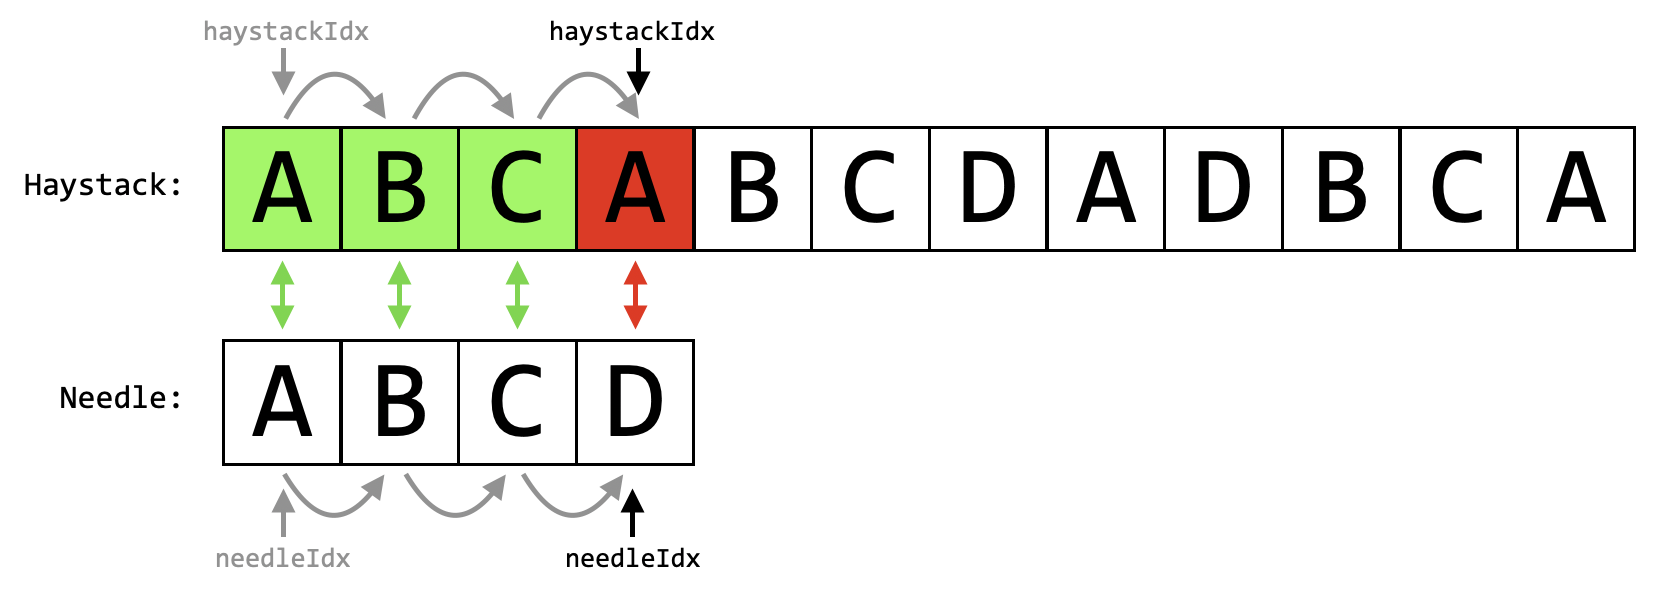
\includegraphics[width=\textwidth]{images/brute_force_1.png}
    \caption{Brute force comparisons up to first mismatch.}
    \label{fig:bf_1}
  \end{minipage}
  \hfill
  \begin{minipage}[b]{0.4\textwidth}
    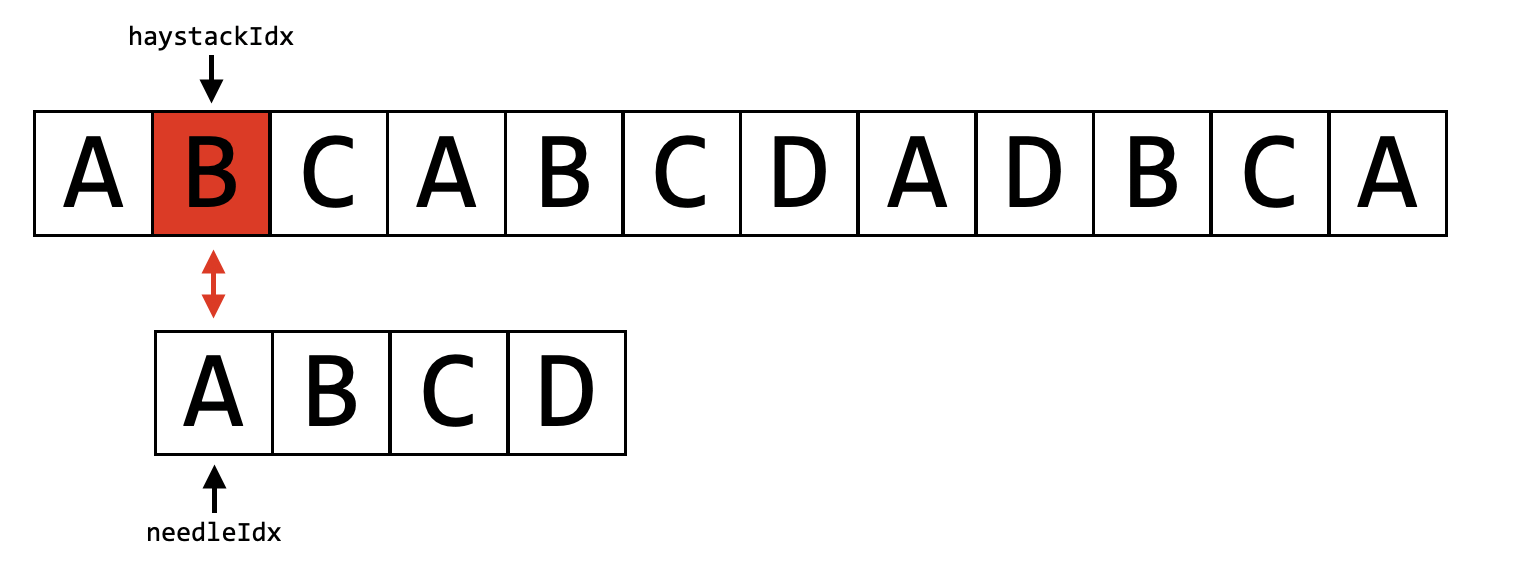
\includegraphics[width=\textwidth]{images/brute_force_2.png}
    \caption{Brute force comparison after first mismatch.}
    \label{fig:bf_2}
  \end{minipage}
\end{figure}
\fi

\subsection*{Python Implementation}

\begin{figure}[h!]
    \centering
    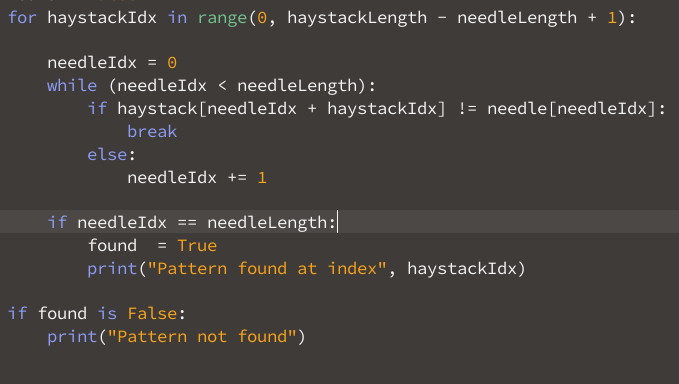
\includegraphics[width=0.50\textwidth]{images/brute_force.png}
    \caption{Code snippet of our brute force implementation}
    \label{fig:bf_code}
\end{figure}

\noindent
The variables \mintinline{Python}{haystackIdx} and \mintinline{Python}{needleIdx} are first initialised to traverse both strings. If a mismatch between these two indices were to occur, then \mintinline{Python}{needleIdx} would reset to 0, and this character would be compared with \mintinline{Python}{haystack[needleIdx + haystackIdx]}. When \mintinline{Python}{needleIdx} traverses the entire needle, then the search pattern has been found and the function prints the index of the haystack at that point.

\subsection*{Analysis}
Let $h, n$ be the length of the haystack and the needle respectively. For a complete search, we would need to go through all characters of the haystack. This means that we need to check $h - n + 1$ substrings. In the inner loop, we would need to compare each character of the needle to each character of the substring of the haystack.

\subsubsection*{Best Case Time Complexity}
In the best case scenario, in the inner loop, the first character is never the same as the first character of the substring, i.e. the first character of the needle does not exist in the haystack. This results in a time complexity of $\mathcal{O}(1)$ in each inner loop, and an overall time complexity of $\mathcal{O}(h-n)$.
 
\subsubsection*{Average Case Time Complexity}
In the case of searching for DNA patterns, there are only four available characters to choose from. The probability of a match is $\frac{1}{4}$. This can be modelled by a geometric distribution $P(X=r) = p(1-p)^{r-1}$, where $X$ is the random variable denoting the number of comparisons that have been after encountering the first mismatch. The probability of having a mismatch is given by $p = 3/4$ and the expected number of mismatches is $E(X) = \frac{1}{p} = \frac{4}{3}$. The Brute Force makes these comparisons $h-n+1$ times. Hence, the average case time complexity can be given by $\frac{4}{3}(h-n+1)$, which is simplified to $\mathcal{O}(h-n)$.

\subsubsection*{Worst Case Time Complexity}
In the worst case, the Brute Force Algorithm would have to traverse through the entire length of the needle making the time complexity $\mathcal{O}(n)$. Hence, the worst case time complexity for brute force is $\mathcal{O}(h - n + 1)(n) = \mathcal{O}(hn)$. There is nothing to analyse for space complexity since we do not need to store any additional data since there is no preprocessing done.

\section*{Knuth-Morris-Pratt (KMP) Algorithm}

\subsection*{Concept}
Figures \ref{fig:kmp_1} and \ref{fig:kmp_2} show an example of how KMP handles a mismatch case by skipping over irrelevant characters to the next occurrence of `A'. This is a key improvement over Brute Force, which only shifts the search pattern by one index with each mismatch. 


\begin{figure}[H]
  \centering
  \begin{minipage}[b]{0.49\textwidth}
    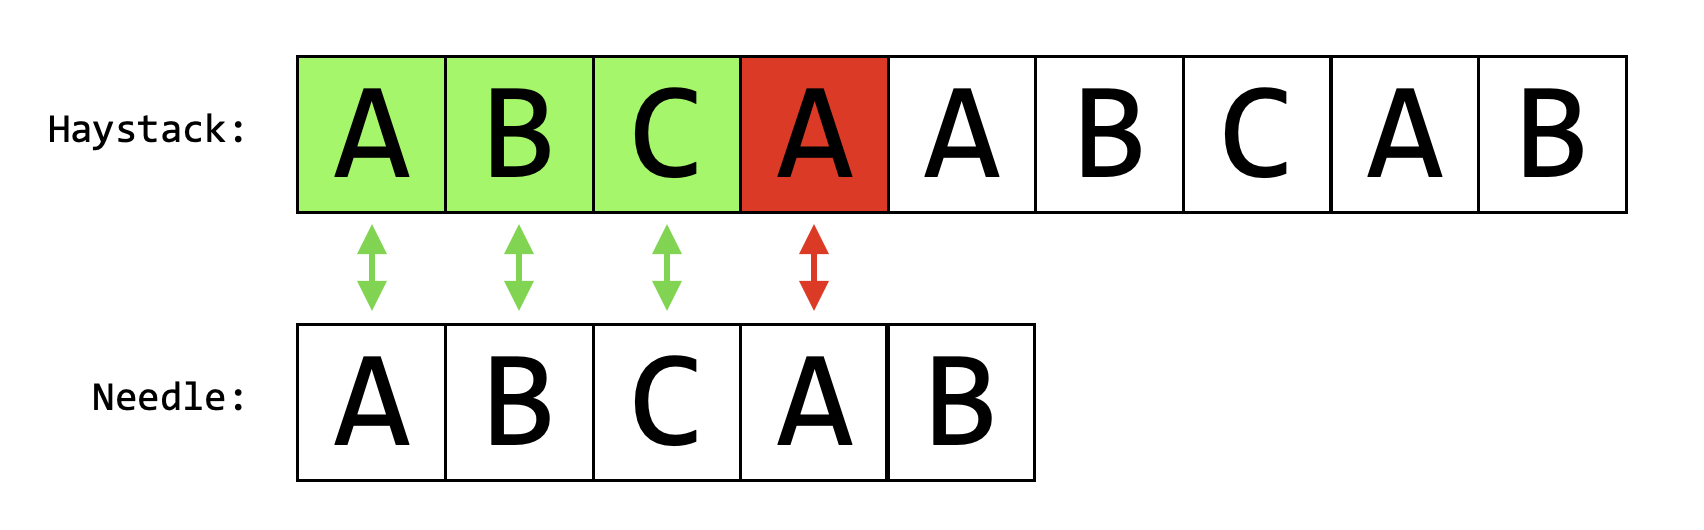
\includegraphics[width=\textwidth]{images/kmp_1.png}
    \caption{Comparisons up to first mismatch.}
    \label{fig:kmp_1}
  \end{minipage}
  \hfill
  \begin{minipage}[b]{0.49\textwidth}
    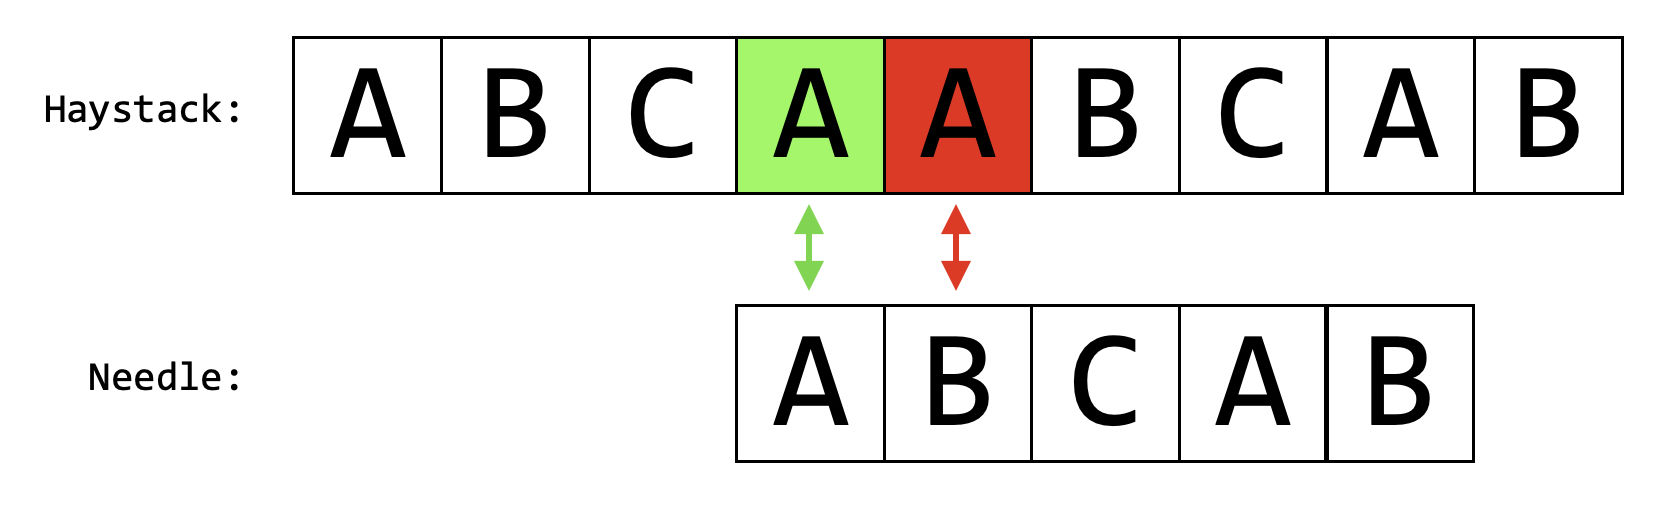
\includegraphics[width=\textwidth]{images/kmp_2.png}
    \caption{Comparison after first mismatch.}
    \label{fig:kmp_2}
  \end{minipage}
\end{figure}

\noindent
In order to facilitate this, the substring first needs to be preprocessed to identify the length of longest recurring patterns within the needle (referred to as prefixes and suffixes). This allows the algorithm to form a table of values that indicate the next index in the haystack that the needle should be compared to. Table \ref{tab:kmp_table} depicts the corresponding lookup table for the example pattern above. If a mismatch occurs at a `A' within the haystack, we are to remain at that index, and compare it with index 1 of the needle. In the same way, if the mismatch occurs at `B', we compare it with index 2 of the needle. In all other cases, we just shift the search pattern right by one increment. 



\begin{table}[H]
    \centering
    \begin{tabular}{llllll}
    1 & 2 & 3 & 4 & 5 \\ \hline
    \multicolumn{1}{|l|}{A} & \multicolumn{1}{l|}{B} & \multicolumn{1}{l|}{C} & \multicolumn{1}{l|}{A} & \multicolumn{1}{l|}{B} \\ \hline
    \multicolumn{1}{|l|}{\textbf{0}} & \multicolumn{1}{l|}{\textbf{0}} & \multicolumn{1}{l|}{\textbf{0}} & \multicolumn{1}{l|}{\textbf{1}} & \multicolumn{1}{l|}{\textbf{2}} \\ \hline
    \end{tabular}
    \caption{KMP Lookup table.}
    \label{tab:kmp_table}
\end{table}

\subsection*{Python Implementation}

The function shown in Figure \ref{fig:kmp_preprocessing} generates \mintinline{Python}{processedNeedle}, which is the KMP lookup table. We calculate the value such that if the \mintinline{Python}{needle[leftCursor]} and \mintinline{Python}{needle[rightCursor]} matches, we increment \mintinline{Python}{leftCursor} and assign this value to the \mintinline{Python}{processedNeedle}, and then increment \mintinline{Python}{rightCursor}. If a mismatch occurs and \mintinline{Python}{leftCursor} is pointing to the first character, we reinitialise it. This constructs an array storing the lengths of all prefix/suffix pairs in the needle. If a mismatch occurs at index $a$, \mintinline{Python}{processedNeedle[a - 1]} gives the index number of the needle that should be used to make the next comparison. 

\begin{figure}[H]
  \centering
  \begin{minipage}[b]{0.49\textwidth}
    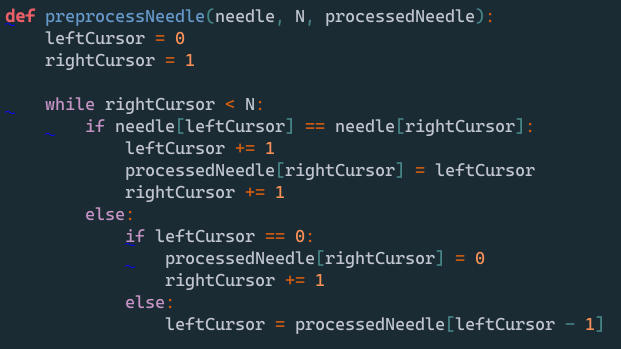
\includegraphics[width=\textwidth]{images/preprocessKMP.png}
    \caption{Preprocess Function for KMP}
    \label{fig:kmp_preprocessing}
  \end{minipage}
  \hfill
  \begin{minipage}[b]{0.49\textwidth}
    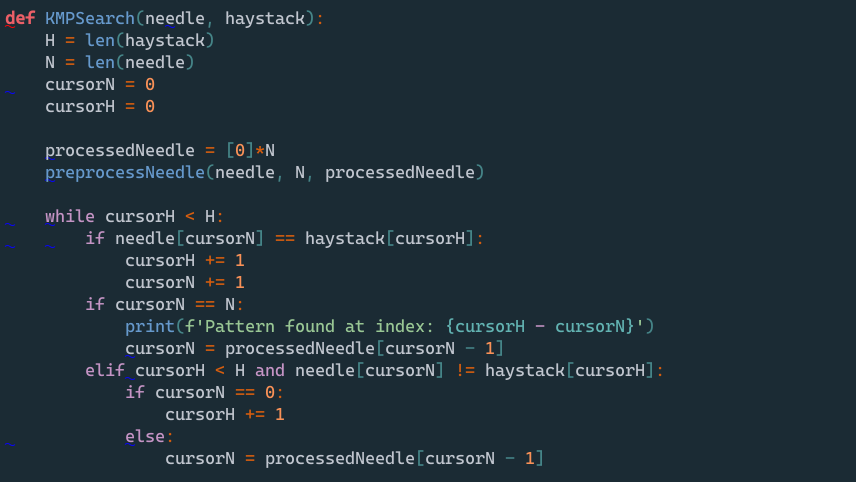
\includegraphics[width=\textwidth]{images/KMP.png}
    \caption{KMP Search Function}
    \label{fig:kmp_search}
  \end{minipage}
\end{figure}

\iffalse
If the mismatch happens at index $a$, this means the first $a-1$ characters are matching. \mintinline{Python}{processedNeedle[a - 1]} is the number of characters that are both the prefix and suffix of that substring of the needle of length a. This information is used as a reference to determine which index to skip to next for comparison.
\fi

\subsection*{Analysis}

%Commented out for now
\iffalse
Since the length of the haystack and needle are $h, n$ respectively, we would begin comparison of the needle and the haystack and increment the value of the cursor while they match. \mintinline{Python}{if cursorN == N} indicates that all characters match with each other and the pattern is found. 
\fi

\subsubsection{Preprocessing Time}
Since we do not need to do the comparison for those that are already matched, we only need to do one comparison for each character in the haystack. This means that the time complexity of the matching will be $\mathcal{O}(h)$. However, time is taken to do the preprocessing. This is done in $\mathcal{O}(n)$ time, because the preprocessing function traverses through the needle to calculate the value of prefix/suffix pairs.

\subsubsection{Time Complexity}
Since the preprocessing and the matching happens linearly, the time complexity of the algorithm is $\mathcal{O}(h+n)$. In the given problem, the best case and worst case time complexity for KMP remains the same, because we want to find all occurrences of the needle in the haystack. Hence, the entire text needs to be traversed, even if a match has previously been found. This means that the best, worst, and average case time complexity remains $\mathcal{O}(h+n)$.

\subsubsection{Space Complexity}
The improvement to a linear time complexity in the worst case from $\mathcal{O}(hn)$ to $\mathcal{O}(h + n)$ comes with a trade-off in space complexity. In the case of brute force, there is no need to store any data. However, the efficiency in KMP comes from the existence of the lookup table which is the array which tells us how many characters we do not need to match. The size of this array is equivalent to the length of the needle that we are searching for. Thus, the space complexity for KMP would be $\mathcal{O}(n)$.

\section*{Empirical Analysis}

As is consistent with our analysis, KMP takes a shorter amount of time compared to Brute Force. Despite the preprocessing time, the time cost of $\mathcal{O}(h+n)$ is generally be more efficient than the worse case of Brute Force ($\mathcal{O}(hn)$).

\begin{figure}[H]
  \centering
  \begin{minipage}[b]{0.49\textwidth}
    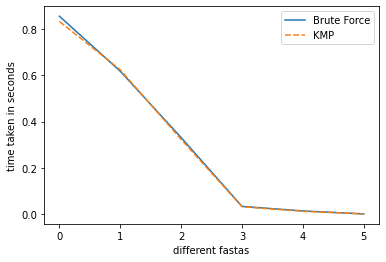
\includegraphics[width=\textwidth]{images/brute-force-best.png} 
    \caption{Brute Force (best case): $\mathcal{O}(h)$ vs. KMP: $\mathcal{O}(h+n)$}
    \label{fig:bf_best}
  \end{minipage}
  \hfill
  \begin{minipage}[b]{0.49\textwidth}
    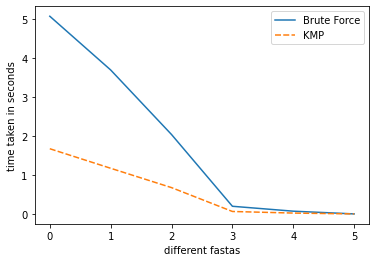
\includegraphics[width=\textwidth]{images/brute-force-worst.png} 
    \caption{Brute Force (worst case): ($\mathcal{O}(hn)$) vs. KMP}
    \label{fig:bf_worst}
  \end{minipage}
\end{figure}

\begin{figure}[H]
    \centering
    \begin{minipage}[b]{0.49\textwidth}
    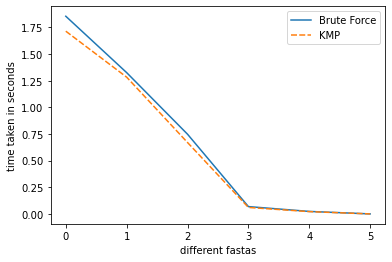
\includegraphics[width=\textwidth]{images/graph.png} 
    \caption{Performance of Brute Force compared to KMP in a realistic scenario}
    \label{fig:graph}
  \end{minipage}
\end{figure}

\noindent
KMP consistently outperforms Brute Force even though some of the improvements were minimal. It can be seen that the performance of Brute Force approaches that of KMP in its best case. Even though the performance of the Brute Force Algorithm is much worse than KMP in its worst case, this scenario is very unlikely to occur in realistic DNA substring searches. We conclude that KMP performs more consistenly, and is therefore more suited for this task.

\iffalse
This may be because the worst case scenario for the Brute Force Algorithm only occurs in the specific case when $n$ comparisons have to be made for every character in the haystack. However, for this particular application in searching for a DNA pattern, the number of comparisons that have to be made would very likely be much less than $n$. This, coupled with the fact that the KMP Algorithm has to perform preprocessing steps on the needle is the reason that the two algorithms have performed so similarly.
\fi

\nocite{geeksforgeeks_kmp}
\nocite{wikipedia_2020}
\nocite{geeksforgeeks_bf}

\section*{References}
% \newpage
% \renewcommand\bibname{References}
\printbibliography[heading=none]
%bib here

 % Link to the chapter tex file

\end{document}
